\label{powerlaw}

\section{Power Law Processes}

\frame[t] {
\frametitle{Power Law Distribution}
A power law distribution is a distribution whose tail falls off as
\[ P(X=x) \propto x^{-\alpha} \]
For some $\alpha > 1$.  The simplest such distribution is the zeta distribution on natural numbers:
\[ f_\alpha(k) = \frac{k^{-\alpha}}{\zeta(\alpha)} \]
and the Pareto distribution on the real line (with small-scale cutoff $x_{min} > 0$):
\[ f_\alpha(x) = \frac{\alpha-1}{x_{min}} \left(\frac{x}{x_{min}}\right)^{-\alpha} \]
}

\frame[t] {
\frametitle{Scale Free Property}
A power law distribution on the real line is {\em scale free} in the sense that, for all scales $k > 0$ and $x > x_{min}$
\[  f_{\alpha}(kx) \propto f_{\alpha}(x) \]
Where the proportionality constant depends only on $k$.
}

\frame[t] {
\frametitle{Power Laws in Nature}
Words in natural language, arranged by frequency \cite{Zipf1965}.
\begin{center}
\includegraphics[scale=0.35]{figs/wikipedia-zipf.png} \\
Log-log plot of word frequency in Wikipedia (source: Wikipedia)
\end{center}
}

\frame[t] {
\frametitle{Power Laws in Nature}
Cities arranged by population \cite{Blank2000}.
}

\frame[t] {
\frametitle{Power Laws in Nature}
Earthquakes arranged by magnitude \cite{Gutenberg1955}. \\
\begin{center}
\includegraphics[scale=0.35]{figs/earthquakes.png} \\
(image source: http://quake.usgs.gov/recenteqs/latest.htm)
\end{center}
}

\frame[t] {
\frametitle{Power Laws in Nature}
Power spectra of natural images \cite{Ruderman1994}.
\begin{center}
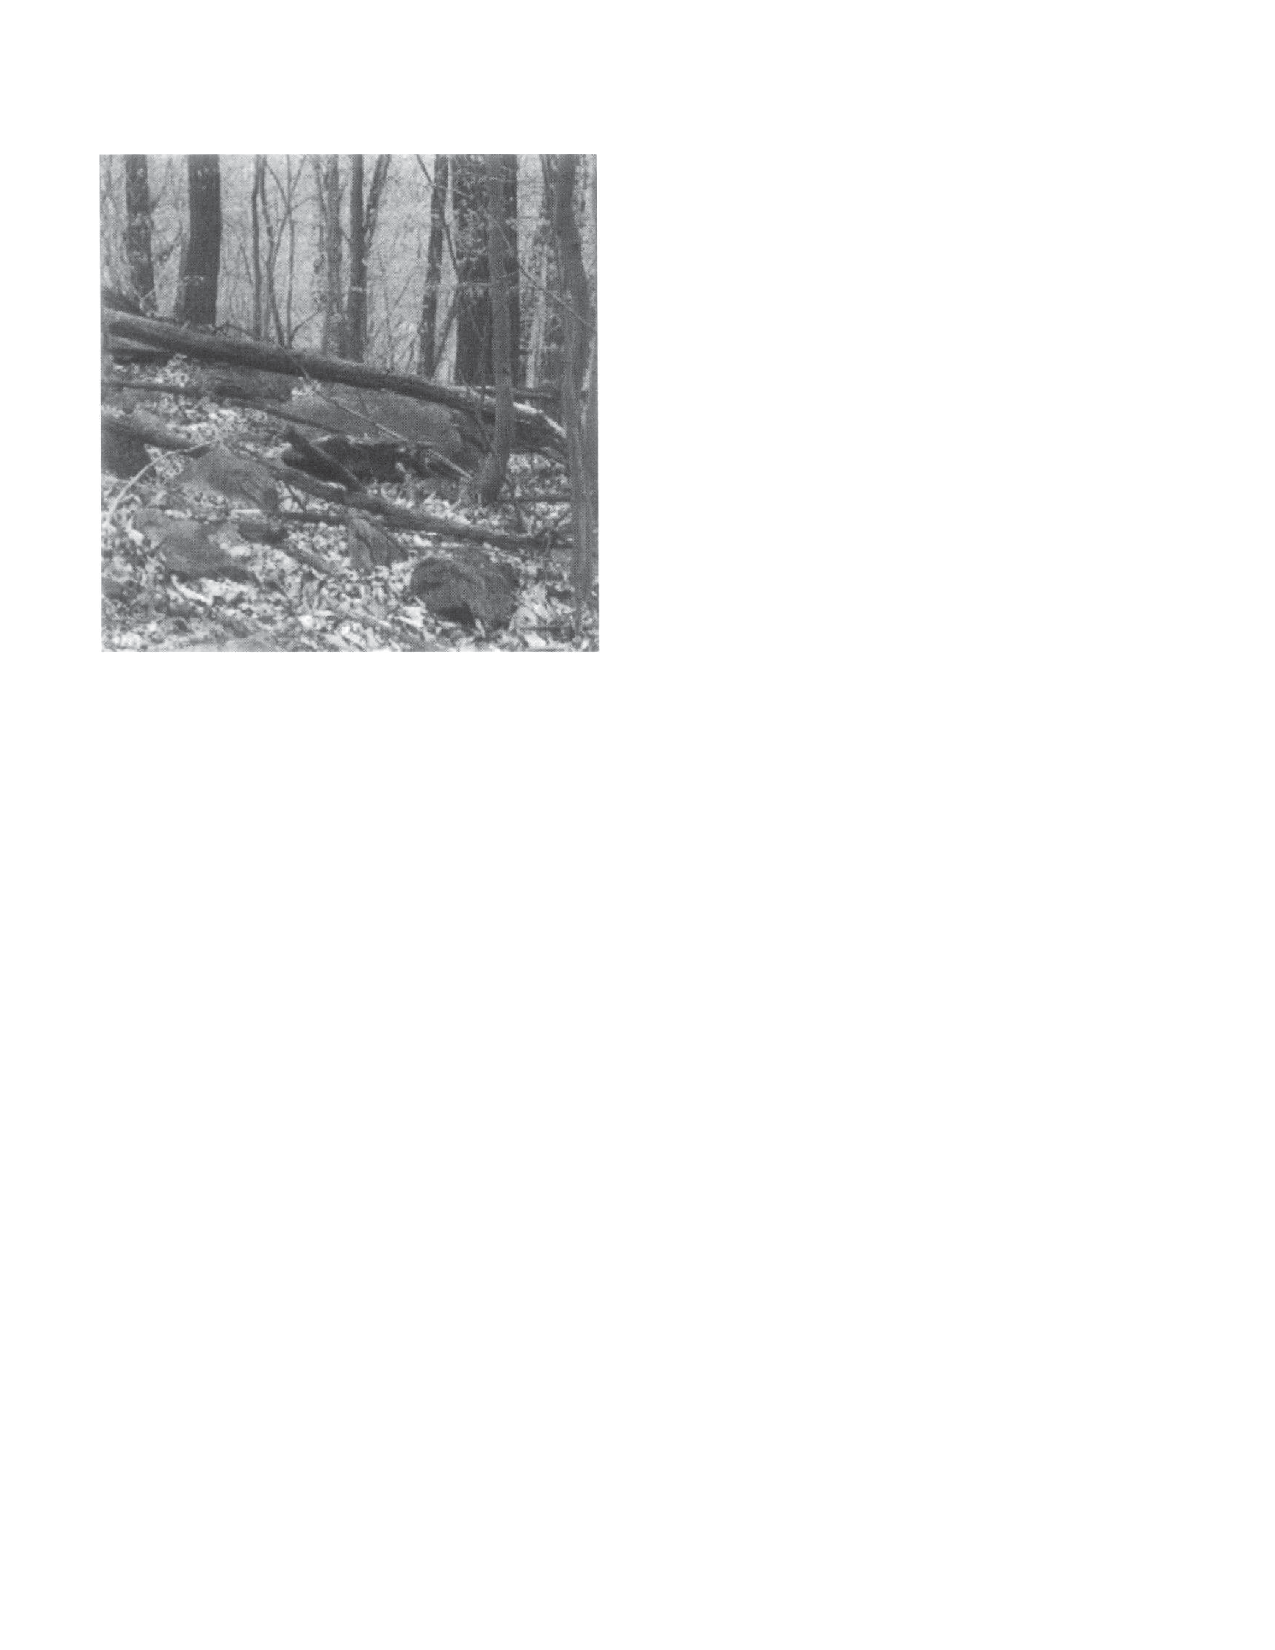
\includegraphics[scale=0.5]{figs/ruderman_bialek_img.pdf}
\hspace*{5 mm}
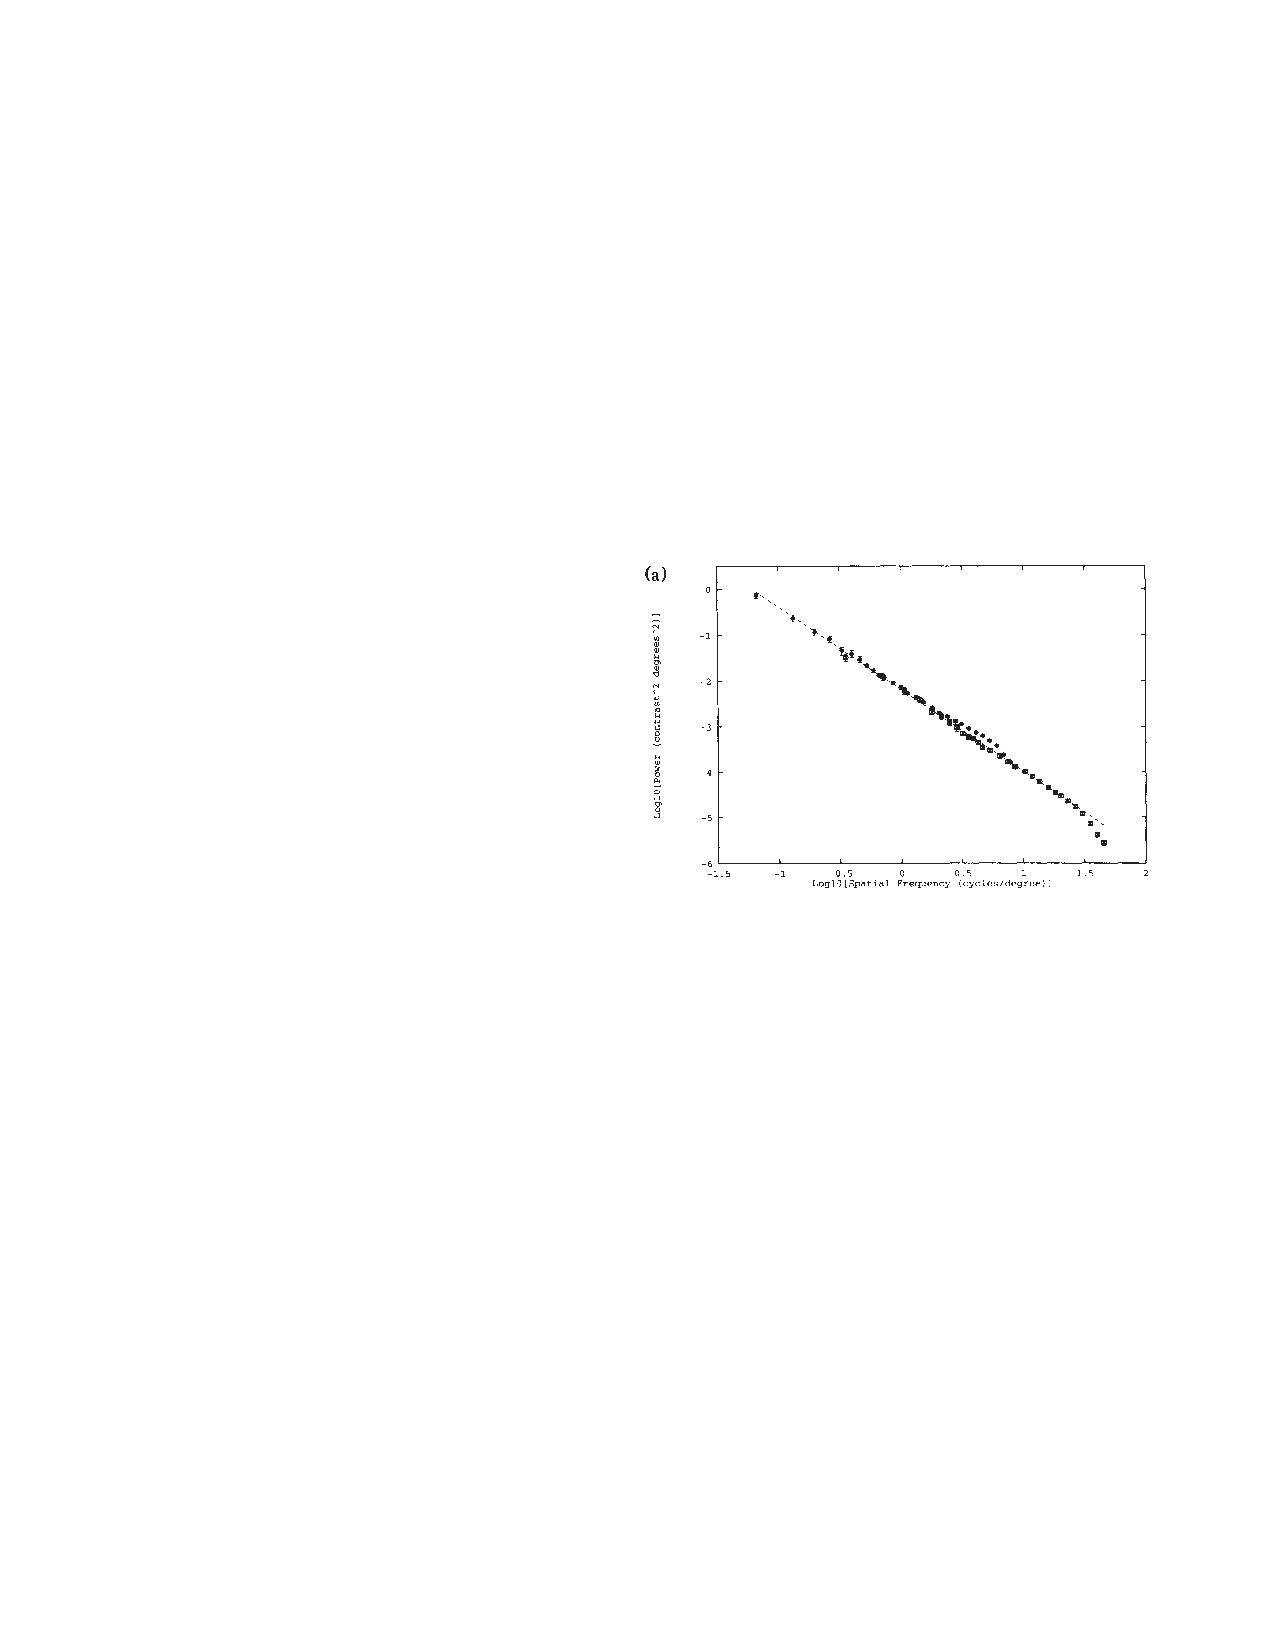
\includegraphics[scale=0.75]{figs/ruderman_bialek_plot.pdf}
\end{center}
}